% =====================================================================
%  Research Statement -- Financial / Mathematical Finance (generic version)
%  Davood Damircheli, Department of Mathematics, Louisiana State University
%  Compile: pdflatex (twice)
%
%  Lines marked  %CHECK  contain claims that should be confirmed before
%  submission (final numbers in in-preparation work, etc.).
%  Deliberately NOT quoted: Asian/barrier accuracy figures (the combined
%  DPG manuscript and Part II disagree) and any table that also appears
%  in another paper.
% =====================================================================
\documentclass[11pt]{article}
\usepackage[letterpaper,hmargin=1in,vmargin=0.85in]{geometry}
\usepackage[T1]{fontenc}
\usepackage{mathpazo}
\usepackage[scaled=0.95]{helvet}
\usepackage{microtype}
\usepackage{amsmath,amssymb}
\usepackage{xcolor}
\usepackage{enumitem}
\usepackage{titlesec}
\usepackage{tikz}
\usetikzlibrary{positioning,arrows.meta,shapes.misc}
\usepackage[hidelinks]{hyperref}

\definecolor{accent}{RGB}{25,70,125}
\definecolor{soft}{RGB}{235,241,248}

\titleformat{\section}{\normalfont\large\bfseries\color{accent}}{\thesection.}{0.5em}{}
\titlespacing*{\section}{0pt}{9pt}{3pt}
\titleformat{\paragraph}[runin]{\normalfont\bfseries}{}{0pt}{}[.]
\titlespacing*{\paragraph}{0pt}{4pt}{0.6em}
\setlist{nosep,leftmargin=1.3em,topsep=2pt}
\setlength{\parskip}{3pt}
\setlength{\parindent}{0pt}

\renewcommand{\ttdefault}{pcr}
\newcommand{\rc}[1]{\textcolor{accent}{[#1]}}

\begin{document}

% ------------------------------------------------------------- header
\begin{center}
{\LARGE\bfseries Research Statement}\\[3pt]
{\large Davood Damircheli}\\[1pt]
{\small Department of Mathematics, Louisiana State University\\
\href{mailto:ddamircheli@lsu.edu}{ddamircheli@lsu.edu} \;$\cdot$\;
\href{https://davooddamircheli.github.io}{\nolinkurl{davooddamircheli.github.io}}}
\end{center}
\vspace{-4pt}

% ------------------------------------------------------------- overview
\section*{Overview}

My research is in computational mathematical finance. I design and analyze
numerical methods for pricing, hedging, and risk under market models that
go beyond geometric Brownian motion: \textbf{jumps and tempered-stable
L\'evy dynamics}, \textbf{regime switching}, \textbf{anomalous
(subdiffusive) price dynamics}, and \textbf{credit-rating migration}. I am
particularly interested in contracts whose value is shaped by a
\textbf{constraint}, such as early exercise, barriers, path dependence, or
default. Realistic dynamics turn the pricing equation into a nonlocal
partial integro-differential equation (PIDE), and the constraint turns it
into a variational inequality or a free-boundary problem. Both features
cause trouble for standard solvers, and that is where most of the
financially relevant information sits: the early-exercise boundary, the
default threshold, and the tails of the jump distribution.

I approach these problems at four connected levels:
\begin{enumerate}[label=(\roman*),leftmargin=2.2em]
\item \emph{analysis of the pricing equation}: well-posedness, coercivity,
      and the structure that makes it stable;
\item \emph{structure-preserving discretization}: methods that keep that
      structure and are proved to converge, for prices \emph{and} Greeks;
\item \emph{calibration to market data}: fitting models to observed option
      prices, testing them across calm and crisis markets, and letting the
      data decide which model and which solver a task needs; and
\item \emph{certified computation}: computable, rigorous bounds that say,
      query by query, whether a fast price---from a reduced model or a
      neural network---is accurate to a stated tolerance, such as one cent.
\end{enumerate}
The last level answers a question that practitioners now face daily as
machine-learned pricers enter production: \emph{when can a fast price be
trusted?} My background combines the two sides of the field. I hold an
M.Sc.\ in Applied and Financial Mathematics, Ph.D.s in Mathematical
Sciences and in Computational Engineering (Mississippi State), and I
worked for two years as a risk analyst at a commercial bank. There I
worked daily with the bank's cash-flow and balance-sheet data to build
liquidity-risk models (gap analysis, liquidity-at-risk, cash-flow-at-risk,
stress testing, expected shortfall), and I applied machine learning
(support-vector machines, $k$-means clustering) to credit-risk analysis.
That experience made me comfortable with real, messy data, and it taught
me that model errors carry costs. Both lessons shape my work: every model
I study is meant to meet data, and every number it produces should come
with a guarantee.

\begin{center}
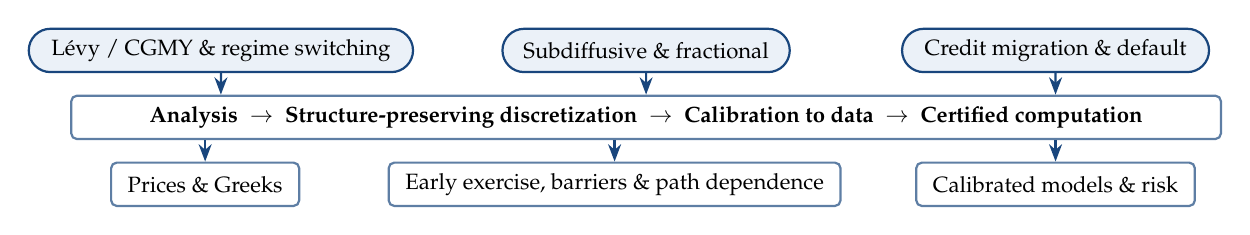
\begin{tikzpicture}[
  font=\footnotesize,
  pill/.style={rounded rectangle, draw=accent, fill=soft, thick, minimum height=5.5mm, inner xsep=7pt},
  box/.style={rectangle, rounded corners=2pt, draw=accent!70, fill=white, thick, minimum height=5.5mm, inner xsep=6pt, align=center},
  arr/.style={-{Stealth[length=2.2mm]}, accent, thick}]
  \node[pill] (lv) at (-5.4,0) {L\'evy / CGMY \& regime switching};
  \node[pill] (fr) at (0,0) {Subdiffusive \& fractional};
  \node[pill] (cr) at (5.2,0) {Credit migration \& default};
  \node[box, minimum width=14.6cm] (lev) at (0,-0.85)
     {\textbf{Analysis} \;$\rightarrow$\; \textbf{Structure-preserving discretization} \;$\rightarrow$\; \textbf{Calibration to data} \;$\rightarrow$\; \textbf{Certified computation}};
  \node[box] (o1) at (-5.6,-1.7) {Prices \& Greeks};
  \node[box] (o2) at (-0.4,-1.7) {Early exercise, barriers \& path dependence};
  \node[box] (o3) at (5.2,-1.7) {Calibrated models \& risk};
  \draw[arr] (lv) -- (lv|-lev.north);
  \draw[arr] (fr) -- (lev.north);
  \draw[arr] (cr) -- (cr|-lev.north);
  \draw[arr] (lev.south -| o1) -- (o1);
  \draw[arr] (lev.south -| o2) -- (o2);
  \draw[arr] (lev.south -| o3) -- (o3);
\end{tikzpicture}
\end{center}
\vspace{-10pt}

% ------------------------------------------------------------- theme 1
\section{Pricing under jumps: tempered-stable and regime-switching L\'evy models}

\paragraph{A structure-preserving Galerkin method for CGMY}
Under the CGMY process the pricing operator contains tempered fractional
derivatives of order $Y\in(0,2)$, which are dense, singular, and nonlocal.
In \rc{S2} I derived exact Fourier-symbol connection coefficients for the
exponentially conjugated tempered Riemann--Liouville operators in a
B-spline basis. The resulting matrices are exactly Toeplitz and are applied
by FFT in $O(N\log N)$. A monotonicity lemma for the symbol gives
$\operatorname{Re}\mathcal A(\xi)\ge r$, so the pricing operator is
\emph{coercive whenever the interest rate is positive}. Splines supported
in the interior make the discrete stiffness an exact Toeplitz section, so
the discrete method inherits the continuous constants. I proved the fully
discrete rate $O(h^{p-Y/2}+\Delta\tau^2)$ for $Y\in(1,2)$. The method prices
American puts in agreement with a Longstaff--Schwartz Monte Carlo
confidence interval.

\paragraph{Calibration to market data}
A pricing method is useful only if the model it solves can be fitted to
the market. In \rc{S2} I therefore took the method to real data. I
calibrated the five CGMY parameters to S\&P\,500 option quotes in three
market regimes (calm, recovery, and crisis), with the
B-spline solver inside the optimization loop. %CHECK description of data/objective
The fitted model reproduces the implied-volatility surface to within about
2.0--2.5 volatility points in the calm and recovery regimes. In the crisis
regime the error is 7.2 points, where only two maturities were available.
The calibrated parameters also carry economic information: the jump
activity $C$ rises about elevenfold in the crisis regime, a quantitative
signature of market stress read directly from option prices. Each
calibration takes a few minutes. The data also guided the choice of
numerical method: a stabilized Gr\"unwald--Letnikov scheme is about six
times faster at calibration-level accuracy, while only the B-spline method
reaches $10^{-4}$ accuracy in price, which hedging and certification
require. This study is the first step of a data program that I am now
expanding to more underlyings, dates, and maturities (\S5).

\paragraph{Default probabilities under regime-switching tempered-stable dynamics}
In structural credit models with a Markov-modulated L\'evy firm value and
synchronous jumps at regime changes, default probabilities solve a coupled
system of PIDEs with a singular jump integral \rc{J5}. I proved that, for
any strictly positive-definite $C^{2n}$ kernel ($n\ge2$), the compensated
jump integral is finite for \emph{every} generalized tempered-stable L\'evy
measure with activity below 2. This family covers variance gamma, CGMY,
KoBoL, and bilateral gamma. Radial-basis collocation is therefore
de-singularized automatically, with no truncation of small jumps or
Brownian approximation. On a variance-gamma model calibrated to three
European issuers (Axa, STMicroelectronics, Soci\'et\'e G\'en\'erale), the
method agrees with an FFT benchmark. Earlier, I developed radial-basis
collocation for American options under regime-switching jump diffusions
\rc{J7}.

% ------------------------------------------------------------- theme 2
\section{Early exercise, barriers, and path dependence}

\paragraph{Space--time methods for American options}
With collaborators in Chile, I co-developed a space--time least-squares
finite element method for the parabolic obstacle problem
$\partial_t u+Lu\ge f,\ u\ge g$, with complementarity \rc{J2,
\emph{IMA J.\ Numer.\ Anal.}\ 2025}. The method covers general
convection--diffusion--reaction operators $L$, including Black--Scholes in
log-price. We introduce the flux and the reaction force (the
early-exercise premium density) as unknowns. This gives a variational
inequality with a symmetric, coercive form, quasi-optimality for any
discrete convex set, and a reliable a~posteriori estimator. Adaptivity in
space and time then follows the free boundary. For the American put it
restores the optimal rate $O((\#\mathcal P)^{-1/2})$, compared with
$O((\#\mathcal P)^{-3/8})$ on uniform meshes.

\paragraph{Minimum-residual (DPG) methods for multi-asset and exotic options}
My engineering dissertation \rc{C1} introduced discontinuous
Petrov--Galerkin methods to option pricing, including American options
solved by semismooth Newton methods on the symmetric positive-definite DPG
system. I have since developed the theory \rc{S3,\,M2}.
\begin{itemize}
\item For the correlated $d$-asset Black--Scholes operator I proved
      \emph{mesh-independent} inf-sup stability for both the primal and
      the ultraweak formulations. The ultraweak result needs no
      compatibility condition. I also constructed a uniformly bounded
      Fortin operator in one dimension, which makes the practical method
      unconditionally stable and quasi-optimal.
\item The Greeks---Delta, Gamma, and cross-Gamma---are read directly from
      the first-order variables, with no numerical differentiation of
      prices. The method reproduces the Margrabe exchange option to within
      0.06\% at the money, and it prices best-of, basket, and spread
      options.
\item For path-dependent contracts I identified the weighted space
      $H^1_z=\{u: zu_z\in L^2\}$ suited to the arithmetic Asian operator,
      whose diffusion degenerates in the interior of the domain. I also
      showed that discrete barrier monitoring is an $L^2$-nonexpansive
      projection, separate from the PDE step. In computations it leaves no
      value outside the knock-out corridor.
\end{itemize}
In a related line, I combine semismooth Newton methods with moving-least-squares
collocation for pricing and sensitivity analysis under generalized mixed
fractional Brownian motion \rc{S4}.

% ------------------------------------------------------------- theme 3
\section{Credit risk, anomalous dynamics, and stochastic boundary problems}

\paragraph{Credit-rating migration as a free-boundary problem}
In the credit-rating migration model of Liang and coauthors, the volatility
of a corporate bond switches when the firm crosses an unknown rating
threshold, so the coefficients depend on the solution itself. I introduced
a \emph{recovered-coefficient} discontinuous Galerkin method \rc{P2}. The
coefficients are evaluated on a recovered state built from local
averaging, the model's own mollifier, and a computable cutoff. This
recovery is Lipschitz into $W^{2,\infty}$ uniformly in the mesh size, has
the exact solution as a fixed point, and switches off for small $h$ and
$\Delta t$. The analysis gives an $O(h^p+\Delta t)$ energy estimate and an
error bound for the location of the migration boundary. Independent
finite-difference computations confirm the results. The method also
separates the error of the discretization from the error of the model. In
the regimes tested, the error from smoothing the rating switch is about
three orders of magnitude larger than the discretization error, so the
model, not the numerics, limits the accuracy of credit spreads.

\paragraph{Subdiffusive markets}
In illiquid markets prices can stay flat for random periods. Modeling the
underlying as geometric Brownian motion time-changed by an inverse
$\alpha$-stable subordinator leads to a time-fractional Black--Scholes
equation. For this equation I developed fractional-order Taylor-wavelet
collocation in which the Riemann--Liouville integrals of the basis are
computed \emph{exactly} through the regularized beta function \rc{J4}. The
same exact-operator approach extends to other time--space fractional
transport problems \rc{J1}.

\paragraph{Stochastic boundary value problems}
Some financial quantities are fixed by conditions at several dates, for
example boundary-linked assets and smoothing or estimation of diffusion
paths. These lead to SDEs with multi-point boundary conditions, whose
solutions anticipate the noise. With A.~Foroush Bastani I developed an
adaptive multiple-shooting method that places shooting points along each
sample path \rc{J6}. We proved that it inherits the strong order of the
underlying stochastic Runge--Kutta integrator, and it is about an order of
magnitude more accurate than the existing methods we compared against.

% ------------------------------------------------------------- theme 4
\section{Certified fast pricing and machine-learned surrogates}

\paragraph{Accept/reject certificates for CGMY surrogates}
Calibration and risk aggregation require thousands of prices per second,
and reduced-order or neural surrogates are increasingly used to supply
them. A surrogate that is accurate on average can still be badly wrong at
an individual query. In \rc{M1} I build query-wise certificates for
reduced-basis and neural (DeepONet, POD-NN) surrogates of the CGMY pricing
PIDE. A L\'evy--Khintchine argument gives a closed-form,
parameter-explicit lower bound on the spectrum, which replaces numerical
eigenvalue checks. Empirical interpolation applied to the one-variable
Fourier symbol, rather than to matrices, gives a certificate whose cost
does not depend on the grid and takes milliseconds to evaluate. In my
experiments, at a one-cent tolerance, the certificate never accepted an
inaccurate price. It rejected every tested neural surrogate, and it
flagged out-of-distribution parameter queries far more precisely than a
rule that rejects queries outside the training box. %CHECK final numbers
It also gave an informative negative result: for one-factor models the
tested neural surrogates were not faster than the solver they replace.
This indicates that certified surrogates are worth their cost in the
multi-query, multi-factor settings targeted below.

\paragraph{Guaranteed bounds for neural solutions of obstacle problems}
Neural solvers for optimal-stopping and free-boundary problems rarely come
with error guarantees. In \rc{P1} I proved and implemented guaranteed error
bounds for neural approximations of parabolic obstacle problems, the PDE
form of American-style contracts. The key step is to certify the
\emph{feasible projection} $\hat v=\max\{v,g\}$ of the network, which never
falls below the payoff. This removes all penetration terms and coercivity
constants, and every integral is evaluated with outward-rounded interval
arithmetic, so the bound holds rigorously. The certificate also
\emph{diagnoses} failures of penalty-based training, such as a collapsed
Lagrange multiplier (exercise premium) near the free boundary.

% ------------------------------------------------------------- future
\section{Research agenda for the next five years}

\paragraph{1. Data-driven, certified calibration under L\'evy and multi-factor models}
I will scale the S\&P\,500 study of \rc{S2} into a systematic empirical
program, with three parts.
\begin{itemize}
\item \emph{Panel calibration.} I will calibrate CGMY, variance-gamma, and
      regime-switching models to large panels of option surfaces across
      indices, single stocks, maturities, and years. The result is a time
      series of calibrated parameters. With it I can study how jump
      activity and tail tempering change across market regimes, and test
      whether they act as early indicators of stress.
\item \emph{Parameter uncertainty.} I will quantify the uncertainty of the
      calibrated parameters (by bootstrap and Bayesian inference) and
      compare model-based fits with data-driven benchmarks such as neural
      implied-volatility models.
\item \emph{Fast calibration with guarantees.} Panel calibration needs
      millions of prices, so I will build parametric surrogates and embed
      a certificate in every step of the calibration loop. A price is used
      only if it is accepted; otherwise the full solver is called. The
      result is calibrated surfaces with a guaranteed pricing error.
\end{itemize}
Methodologically, the goals are extension to multi-asset and multivariate
L\'evy models by tensor B-splines and low-rank formats, and a convergence
theory for American options under CGMY. That theory is open because the
discrete operator is not an M-matrix.

\paragraph{2. Certified early-exercise boundaries and Greeks}
Hedging depends on the free boundary and on the Greeks, not only on the
price. I will develop a~posteriori bounds for the early-exercise boundary
and for Greeks obtained from first-order (DPG and least-squares)
variables. I will also design neural optimal-stopping architectures that
respect the payoff constraint by construction. Their training loss will be
a minimum-residual functional, so that its value is itself an error bound.

\paragraph{3. Credit and counterparty risk with free boundaries}
Planned extensions of the migration model include several rating classes
and stochastic interest rates (two- and three-dimensional free-boundary
problems), joint analysis of the smoothing limits, and first-passage
default under regime-switching L\'evy dynamics. That last extension goes
beyond the default-at-maturity setting of \rc{J5}. I will calibrate these
models to data, namely rating-transition histories, corporate-bond
spreads, and CDS quotes, so that the migration thresholds and regime
parameters are estimated rather than assumed. Building on my banking
experience, I also plan to compute liquidity and tail-risk measures
(expected shortfall, liquidity-at-risk) under jump models fitted to data,
with certified error.

\paragraph{4. Non-Markovian and rough dynamics}
My fractional-in-time methods \rc{J4,\,S4} are a natural starting point
for path-dependent pricing equations arising from rough and fractional
volatility. In these equations, memory kernels play the role that tempered
fractional operators play in space for L\'evy models.

\paragraph{Funding, students, and teaching}
These directions fit NSF DMS (Computational Mathematics, Applied
Mathematics, CAREER). They also suit industry partnerships with
quantitative-research and model-validation groups, which need tested,
auditable pricing code. The work offers projects at every level.
Undergraduate and master's students in financial mathematics can start
with calibration studies on real option and credit data, Greeks, or Monte
Carlo benchmarks. Doctoral students can work on certification theory,
L\'evy PIDEs, or free-boundary analysis. I work in Python, R, MATLAB, and
C++, and I release code openly (e.g., \texttt{dpg-finance} in C++/MFEM and
\texttt{certified-neural-obstacle}). I have taught Financial Mathematics,
Financial Management, and Business Calculus. I would welcome teaching
computational finance with hands-on work on market data, numerical
methods for SDEs and PDEs, stochastic calculus, and data science for
finance. I will continue my collaborations with M.~Razzaghi (Mississippi
State), T.~F\"uhrer and M.~Karkulik (Chile), A.~Foroush Bastani (IASBS),
and T.~N.~Vo (Bath). My postdoctoral work with R.~Lipton (LSU) on nonlocal
fracture and large-scale three-dimensional simulation \rc{J3,\,S5} adds
expertise in nonlocal operators and high-performance computing that
carries over directly to high-dimensional pricing.

% ------------------------------------------------------------- references
\vspace{-4pt}
\section*{Cited work {\normalfont\small(labels match my CV)}}
{\footnotesize
\setlength{\parskip}{0pt}
\begin{list}{}{\leftmargin=2.4em\labelwidth=2.1em\labelsep=0.3em\itemsep=0pt\parsep=0pt}
\item[\rc{J1}] D.~Damircheli, M.~Razzaghi, Time--space collocation based on fractional-order generalized Chebyshev wavelets for fractional advection problem, \emph{J.\ Comput.\ Appl.\ Math.}\ (2026) 117776.
\item[\rc{J2}] J.~J.~Carvajal, D.~Damircheli, T.~F\"uhrer, F.~Fuica, M.~Karkulik, A space--time finite element method for parabolic obstacle problems, \emph{IMA J.\ Numer.\ Anal.}\ (2025).
\item[\rc{J3}] S.~Coskun, D.~Damircheli, R.~Lipton, Quasi-brittle fracture: the blended approach, \emph{J.\ Mech.\ Phys.\ Solids} 205 (2025) 106302.
\item[\rc{J4}] D.~Damircheli, M.~Razzaghi, A wavelet collocation method for fractional Black--Scholes equations by subdiffusive model, \emph{Numer.\ Methods PDEs} 40(5) (2024) e23103.
\item[\rc{J5}] D.~Damircheli, M.~Razzaghi, S.-M.-M.~Kazemi, A.~Foroush~Bastani, A de-singularized meshfree approach to default probability estimation under a regime-switching synchronous-jump tempered stable L\'evy model, \emph{Eng.\ Anal.\ Bound.\ Elem.}\ (2023).
\item[\rc{J6}] A.~Foroush~Bastani, D.~Damircheli, An adaptive algorithm for solving stochastic multi-point boundary value problems, \emph{Numer.\ Algorithms} 74 (2017) 1119--1143.
\item[\rc{J7}] A.~Foroush~Bastani, Z.~Ahmadi, D.~Damircheli, A radial basis collocation method for pricing American options under regime-switching jump-diffusion models, \emph{Appl.\ Numer.\ Math.}\ 65 (2013) 79--90.
\item[\rc{C1}] D.~Damircheli, M.~Bhatia, Solution approaches and sensitivity analysis of variational inequalities, \emph{AIAA SciTech} (2019).
\item[\rc{S2}] D.~Damircheli, A B-spline Galerkin method for option pricing under the CGMY tempered stable process, submitted to \emph{SIAM J.\ Financial Math.}; arXiv:2610.07554.
\item[\rc{S3}] D.~Damircheli, DPG methods for linear Black--Scholes option pricing I: European and multi-asset extensions, submitted to \emph{Comput.\ Math.\ Appl.}
\item[\rc{S4}] D.~Damircheli, S.-M.-M.~Kazemi, A semismooth Newton-based non-cardinal MLS collocation method for option pricing and sensitivity analysis under generalized mixed fractional Brownian motion, submitted to \emph{Appl.\ Numer.\ Math.}
\item[\rc{S5}] D.~Bhattacharya, D.~Damircheli, R.~Lipton, Crushing, comminution and fracture: extreme particle deformation in 3D granular aggregates, submitted; arXiv:2506.05362.
\item[\rc{P1}] D.~Damircheli, Certified neural approximations for parabolic obstacle problems, preprint, arXiv:2610.24202 (2026).
\item[\rc{P2}] D.~Damircheli, Recovered-coefficient discontinuous Galerkin approximation of an averaged-state credit-rating migration PDE, preprint, arXiv:2107.09248 (2026).
\item[\rc{M1}] D.~Damircheli, Residual certification of neural and reduced surrogates for tempered-fractional CGMY pricing PIDEs, in preparation.
\item[\rc{M2}] D.~Damircheli, DPG methods for linear Black--Scholes option pricing II: Asian and barrier options, in preparation.
\end{list}
}

\end{document}
